% PLEASE USE THIS FILE AS A TEMPLATE
% Check file iosart2c.tex for more examples
%
% Journal:
%   Journal of Ambient Intelligence and Smart Environments (jaise)
%   Web Intelligence and Agent Systems: An International Journal (wias)
%   Semantic Web: Interoperability, Usability, Applicability (SW)
% IOS Press
% Latex 2e

% options: jaise|wias|sw
% add. options: [seceqn,secfloat,secthm,crcready,onecolumn]


\documentclass{iosart2c}

%\documentclass[sw]{iosart2c}
%\documentclass[wias]{iosart2c}
%\documentclass[jaise]{iosart2c}

\usepackage[T1]{fontenc}
\usepackage{times}%
\usepackage{natbib}% for bibliography sorting/compressing
%\usepackage{amsmath}
%\usepackage{endnotes}
\usepackage{graphics}

%%%%%%%%%%% Put your definitions here
\usepackage[utf8]{inputenc}
\usepackage[hyphens]{url}
\usepackage{verbatim} 
\usepackage[pdftex,urlcolor=black,colorlinks=true,linkcolor=black,citecolor=black]{hyperref}
\def\sectionautorefname{Section}
\def\subsectionautorefname{Subsection}

%% Define a new 'smallurl' style for the package that will use a smaller font.
\makeatletter
\def\url@smallurlstyle{%
  \@ifundefined{selectfont}{\def\UrlFont{\sf}}{\def\UrlFont{\scriptsize\ttfamily}}}
\makeatother
%% Now actually use the newly defined style.
\urlstyle{smallurl}
\newcommand{\nofootnote}[1]{~#1}

%%%%%%%%%%% End of definitions

\pubyear{0000}
\volume{0}
\firstpage{1}
\lastpage{1}

\begin{document}

\begin{frontmatter}

\pretitle{What'chu talkin' about, Willis?}
\title{A Comparison of Conversation Topics\\on Facebook and Twitter}
%\subtitle{}

%\footnote{\url{http://en.wikipedia.org/wiki/Diff'rent\_Strokes\#Later\_appearances\_of\_the\_characters}}

\runningtitle{A Comparison of Conversation Topics on Facebook and Twitter}

%\review{}{}{}

% Two or more authors:
\author[A]{\fnms{Thomas} \snm{Steiner}\thanks{T. Steiner is partially supported by the European Commission under Grant No. 248296 FP7 I-SEARCH project}},
\author[B]{\fnms{Arnaud} \snm{Brousseau}\thanks{A. Brousseau was an intern at Google Germany GmbH at the time of writing.}},
\author[C]{\fnms{Raphaël} \snm{Troncy}},
\author[D]{\fnms{Ruben} \snm{Verborgh}},
\author[E]{\fnms{Rik} \snm{Van de Walle}},
\author[F]{\fnms{Joaquim} \snm{Gabarró Vallés}}

\runningauthor{T. Steiner, A. Brousseau, R. Troncy, R. Verborgh, R. Van de Walle, J. Gabarró}

\address[A]{Google Germany GmbH, ABC-Str. 19, 20354 Hamburg, Germany,\\
E-mail: tomac@google.com}
\address[B]{Google Germany GmbH, ABC-Str. 19, 20354 Hamburg, Germany,\\ 
E-mail: arnaud.brousseau@gmail.com}
\address[C]{EURECOM, Sophia Antipolis, France\\
E-mail: raphael.troncy@eurecom.fr}
\address[D]{Ghent University -- IBBT, ELIS, Multimedia Lab, Gaston Crommenlaan 8/201, 9050 Ghent, Belgium,\\
E-mail: ruben.verborgh@ugent.be}
\address[E]{Ghent University -- IBBT, ELIS, Multimedia Lab, Gaston Crommenlaan 8/201, 9050 Ghent, Belgium,\\
E-mail: rik.vandewalle@ugent.be}
\address[F]{Universitat Polit\`{e}cnica de Catalunya, Department LSI, 08034 Barcelona, Spain,\\
E-mail: gabarro@lsi.upc.edu}

\begin{abstract}
\begin{comment}
The Twitter Trends feature allows for a global or local view on ``what's happening in my world right now" from a tweet authors' point of view. In this paper, we show the possibility to complete the functionality provided by Twitter Trends via having a closer look at the other side: the tweet readers' point of view. While Twitter Trends works by analyzing the frequency of terms and their velocity of appearance in tweets being authored, our approach is based on the popularity of extracted named entities (in the sense of Linked Data) in tweets being read. Our experimentation architecture uses a client-side browser extension to harvest and dissect tweets from users' timelines, search result pages, or profile pages. Named entities are extracted via several third-party Natural Language Processing (NLP) Web services in parallel, and are then reported to a Web analytics framework, which is used to store, analyze, and compute trends by pivoting the reported named entities by Web analytics data, e.g., users' geographic locations.
\end{comment}
In recent years, social media mining has become an essential tool for marketers, traders, and researchers. The information people share publicly on social networks harbors tremendous amounts of valuable social data. Social networks today are very much ``walled gardens'', excellently illustrated by David Simonds' cartoon~(\autoref{fig:DavidSimonds}~\cite{DavidSimonds}).

\end{abstract}

\begin{keyword}
 \sep
\end{keyword}

\end{frontmatter}

%%%%%%%%%%% The article body starts:

\section{Introduction}

% I DON'T WORK
\begin{comment}
\begin{figure}
\centering
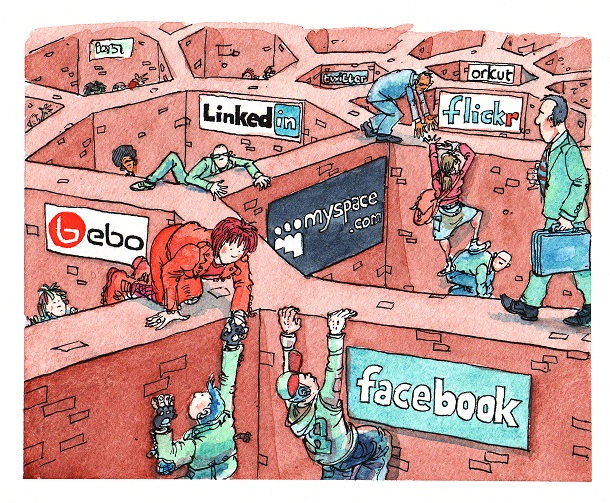
\includegraphics[width=1.0\linewidth]{./resources/davidsimonds.png}
\caption{Social networks as walled gardens.}
\label{fig:DavidSimonds}
\end{figure}
\end{comment}

%%%%%%%%%%% The bibliography starts:
\bibliographystyle{abbrv}
\bibliography{swj2012}

\end{document}
